\section{Auswertung}
\label{sec:Auswertung}

\begin{figure}
  \centering
  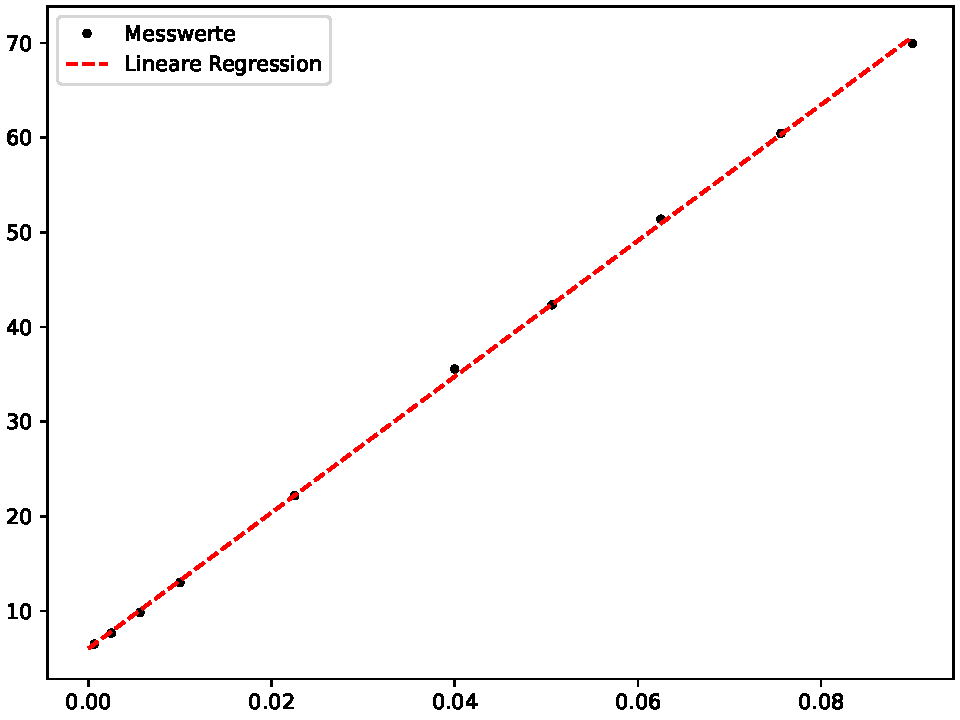
\includegraphics{plot.pdf}
  \caption{Plot.}
  \label{fig:plot}
\end{figure}




\begin{table}[http]
  \centering
  \caption{In dieser Tabelle ist die gemessene Sink- und Steigzeit von den ersten vier Öltröpchen eingetragen.}
  \label{tab:Tabelle}
  \sisetup{table-format=1.1, per-mode=reciprocal}
  \begin{minipage}[t]{0.2\linewidth}
    \begin{tblr}[t]{
      colspec = {S[table-format=1.2] S[table-format=1.2] },
      row{1} = {guard, mode=math},
    }
    \toprule
    t_{sink} \mathbin{/} \unit{\second} & t_{steig} \mathbin{/} \unit{\second}  \\
    \midrule
    1.61  &  1.48 \\
    1.87  &  1.40 \\
    1.13  &  1.57 \\
    1.35  &  1.36 \\
    1.43  &  1.54 \\
    1.15  &  1.38 \\
    1.55  &  1.45 \\

    \bottomrule
  \end{tblr}
\end{minipage}
\hfill
\begin{minipage}[t]{0.2\linewidth}
    \begin{tblr}[t]{
      colspec = {S[table-format=1.2] S[table-format=1.2] },
      row{1} = {guard, mode=math},
    }
    \toprule
    t_{sink} \mathbin{/} \unit{\second} & t_{steig} \mathbin{/} \unit{\second}  \\
    \midrule
    2.28  &  2.37 \\
    2.43  &  2.41 \\
    2.21  &  2.40 \\
    2.65  &  2.06 \\
    2.44  &  2.73 \\
    \bottomrule
  \end{tblr}
\end{minipage}
\hfill
\begin{minipage}[t]{0.2\linewidth}
  \begin{tblr}[t]{
    colspec = {S[table-format=1.2] S[table-format=1.2] },
    row{1} = {guard, mode=math},
  }
  \toprule
  t_{sink} \mathbin{/} \unit{\second} & t_{steig} \mathbin{/} \unit{\second}  \\
  \midrule
  2.97  &  2.70 \\
  2.50  &  2.93 \\
  2.42  &  2.66 \\
  2.63  &  2.95 \\
  2.58  &  2.79 \\

  \bottomrule
\end{tblr}
\end{minipage}
\hfill
\begin{minipage}[t]{0.2\linewidth}
    \begin{tblr}[t]{
      colspec = {S[table-format=1.2] S[table-format=1.2] },
      row{1} = {guard, mode=math},
    }
    \toprule
    t_{sink} \mathbin{/} \unit{\second} & t_{steig} \mathbin{/} \unit{\second}  \\
    \midrule
    2.18  &  3.11 \\
    2.70  &  3.03 \\
    3.21  &  2.72 \\
    2.55  &  3.10 \\
    2.44  &  2.89 \\
    \bottomrule
  \end{tblr}
\end{minipage}
\end{table}

\begin{table}[http]
  \centering
  \caption{Hier ist die Sink- und Steigzeit von den Öltröpchen 5 bis 7 eingetragen.}
  \label{tab:Tabelle}
  \sisetup{table-format=1.1, per-mode=reciprocal}
  \begin{minipage}[t]{0.3\linewidth}
    \begin{tblr}[t]{
      colspec = {S[table-format=1.2] S[table-format=1.2] },
      row{1} = {guard, mode=math},
    }
    \toprule
    t_{sink} \mathbin{/} \unit{\second} & t_{steig} \mathbin{/} \unit{\second}  \\
    \midrule
    3.59  &  4.64 \\
    3.62  &  4.93 \\
    3.74  &  4.61 \\
    3.73  &  4.96 \\
    3.88  &  4.63 \\

    \bottomrule
  \end{tblr}
\end{minipage}
\hfill
\begin{minipage}[t]{0.3\linewidth}
    \begin{tblr}[t]{
      colspec = {S[table-format=1.2] S[table-format=1.2] },
      row{1} = {guard, mode=math},
    }
    \toprule
    t_{sink} \mathbin{/} \unit{\second} & t_{steig} \mathbin{/} \unit{\second}  \\
    \midrule
    2.26  &  2.98 \\
    2.45  &  3.31 \\
    2.34  &  3.16 \\
    2.39  &  2.83 \\
    2.40  &  3.55 \\
    \bottomrule
  \end{tblr}
\end{minipage}
\hfill
\begin{minipage}[t]{0.3\linewidth}
  \begin{tblr}[t]{
    colspec = {S[table-format=1.2] S[table-format=1.2] },
    row{1} = {guard, mode=math},
  }
  \toprule
  t_{sink} \mathbin{/} \unit{\second} & t_{steig} \mathbin{/} \unit{\second}  \\
  \midrule
  4.73  &  4.98 \\
  4.91  &  4.86 \\
  4.56  &  5.69 \\
  4.39  &  6.72 \\
  4.82  &  5.38 \\

  \bottomrule
\end{tblr}
\end{minipage}
\end{table}


\begin{table}[http]
  \centering
  \caption{In der Tabelle ist die gemessene Sink- und Steigzeit von den letzten drei Öltröpchen aufgeführt.}
  \label{tab:Tabelle}
  \sisetup{table-format=1.1, per-mode=reciprocal}
  \begin{minipage}[t]{0.3\linewidth}
    \begin{tblr}[t]{
      colspec = {S[table-format=1.2] S[table-format=1.2] },
      row{1} = {guard, mode=math},
    }
    \toprule
    t_{sink} \mathbin{/} \unit{\second} & t_{steig} \mathbin{/} \unit{\second}  \\
    \midrule
    4.35  &  8.69 \\
    5.90  &  7.87 \\
    5.99  &  8.48 \\
    5.62  &  7.72 \\
    5.89  &  6.64 \\

    \bottomrule
  \end{tblr}
\end{minipage}
\hfill
\begin{minipage}[t]{0.3\linewidth}
    \begin{tblr}[t]{
      colspec = {S[table-format=1.2] S[table-format=1.2] },
      row{1} = {guard, mode=math},
    }
    \toprule
    t_{sink} \mathbin{/} \unit{\second} & t_{steig} \mathbin{/} \unit{\second}  \\
    \midrule
    3.19  &  4.55 \\
    3.86  &  4.48 \\
    3.63  &  4.31 \\
    3.71  &  4.39 \\
    3.96  &  4.65 \\
    \bottomrule
  \end{tblr}
\end{minipage}
\hfill
\begin{minipage}[t]{0.3\linewidth}
  \begin{tblr}[t]{
    colspec = {S[table-format=1.2] S[table-format=2.2] },
    row{1} = {guard, mode=math},
  }
  \toprule
  t_{sink} \mathbin{/} \unit{\second} & t_{steig} \mathbin{/} \unit{\second}  \\
  \midrule
  6.11  &   8.74 \\
  7.73  &   9.92 \\
  6.84  &   9.79 \\
  7.26  &   9.99 \\
  6.44  &  11.22 \\

  \bottomrule
\end{tblr}
\end{minipage}
\end{table}




Mit der Formel 
\begin{equation}
  \bar{t}=\frac{1}{n} \sum_{i=1}^n t_i
\end{equation}
wird der Mittelwert ausgerechnet.

Siehe \autoref{fig:plot} und \autoref{tab:tabelle}!
